\documentclass[a0paper, 20pt, margin=1in, innermargin=0.0in, blockverticalspace=-0.25in, portrait]{tikzposter}
\usepackage{anyfontsize}
\usepackage{amsmath} % Align eqs and matrix environments
\usepackage{IEEEtrantools} % Better alignment with IEEEeqnarray
\usepackage{gensymb} % Create degrees symbol
\usepackage{siunitx}
\sisetup{
	propagate-math-font = true,
	reset-math-version = false
}
\usetikzlibrary {arrows.meta} % library of arrow symbols
\usepackage{uc-theme}

\usetikzlibrary{positioning}

% set theme parameters
\tikzposterlatexaffectionproofoff  % turn off tikzposter watermark
\usetheme{UCTheme}
\usecolorstyle{UCStyle}

\title{
	\parbox{\linewidth}{\centering
		ESTABLISHMENT OF VLBI BETWEEN THE GTM AND SEVERAL POSSIBLE  RADIOTELESCOPES: ZELENCHUK, GREEN BANK, PUSHINO, PARKES, AND ALMA \\
		\vspace{1em}
		COSPAR GENERAL ASSEMBLY \\
		MOSCOW, RUSSIA, AUGUST 2014 \\
		\vspace{1em}
	}
}
\author{
	Victor I. Krilov 
	(Department of Astronomy and Cosmic Geodesy, Moscow State University of Geodesy and Cartography),\\
	Tatiana N. Kokina and Daniel Mendoza-Araiza
	(Center for Astronomy, Autonomous University of Sinaloa UAS),\\
	Julio Saucedo-Morales 
	(Department for Research in Physics, University of Sonora UNISON),\\
	Daniel Flores-Gutierrez 
	(Institute of Astronomy, UNAM).
}

\begin{document}

\maketitle

% Logos
\node[anchor=north west,yshift=-17pt] at (TP@title.north west)
	{
\includegraphics[width=0.10\textwidth]{Figures/cospar_moscow_2014.png}};

\node[anchor=south west,yshift=1em] at (TP@title.south west)
	{
\includegraphics[width=0.09\textwidth]{Figures/UAS_logo.png}};

\node[anchor=north east,yshift=-17pt] at (TP@title.north east)
	{
\includegraphics[width=0.10\textwidth]{Figures/miigaik_logo.png}};

\node[anchor=south east,yshift=1.5em] at (TP@title.south east)
	{
\includegraphics[width=0.10\textwidth]{Figures/UNISON_logo.png}};

% Body text
\begin{columns}

 % First column
\column{0.5}% Width set relative to text width

\block{}{
Very Large Base Interferometry is a powerful means to determine the Earth's rotational parameters and to do basic research on
lithospheric plaques derive,
marea phenomena,
as well as on the motion of the poles,
among others.
But it can also provide useful data to solve various geophysical problems.
The work presented here is about a problem of both great current interest to Mexican science,
while at the same time it may potentially have a significant impact to the Mexican economy.
\vspace{1em}

The Mexican National Geodetic Network (Red Geodésica Nacional, Fig.~1) is linked through NAVSTAR (GPS) (Fig.~2) to the International System of Coordinates ITRF (Fig.~3),
but the presence of seismic activity in most places of Mexico makes it highly desirable to contribute with a point to the ITRF in order to have an even more rigid network for the study of seismic phenomena.
Here we explore the possibility of achieving this with the LMT as a VLBI station.
}

% Images
\begin{subcolumns}
	% Left column images
	\subcolumn{0.5} 
	\block{}{
		\normalsize
		\node[anchor=north west] (rgna)
			{
				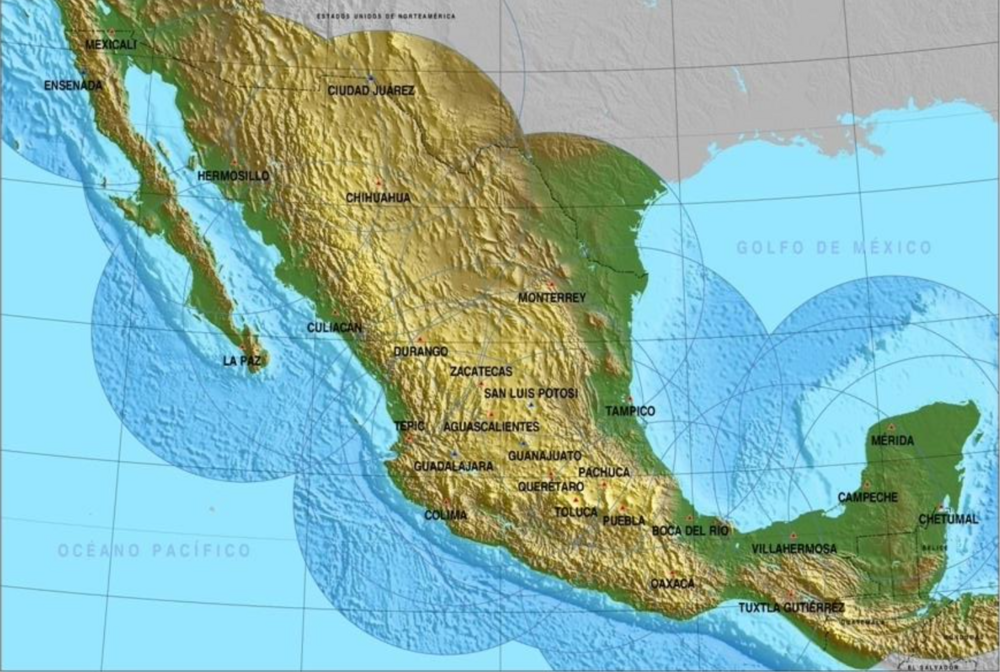
\includegraphics[width=0.20\textwidth]{Figures/RGNA.png}
			};
		\node (cap1) [below=0cm of rgna,xshift=2.7em,yshift=1.5em] {\textbf{Fig. 1}};
		\vspace{1em}
	  %
		\node (itrf) [below=0.5cm of cap1,xshift=2.7em]
			{
				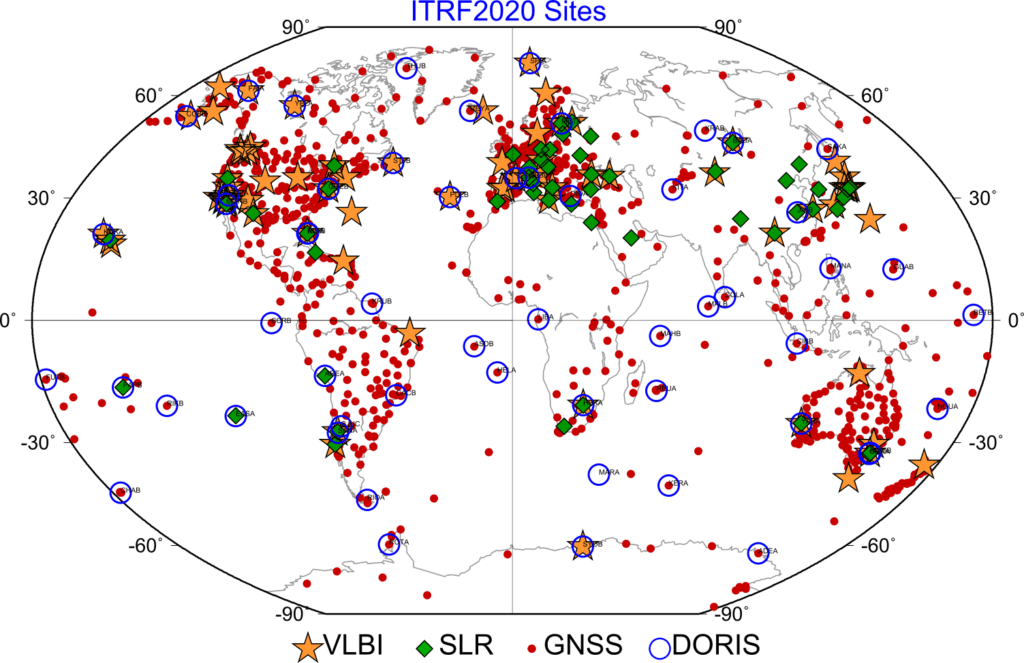
\includegraphics[width=0.20\textwidth]{Figures/ITRF_2020.png}
			};
		\node (cap3) [below=0cm of itrf,xshift=2.7em,yshift=1.5em] {\textbf{Fig. 3}};
	  %		
		\vspace{1em}
	} 
	% Right column images
	\subcolumn{0.5} 
	\block{}{
		\normalsize
		\begin{center}
			\node[anchor=north west] (gps) {
				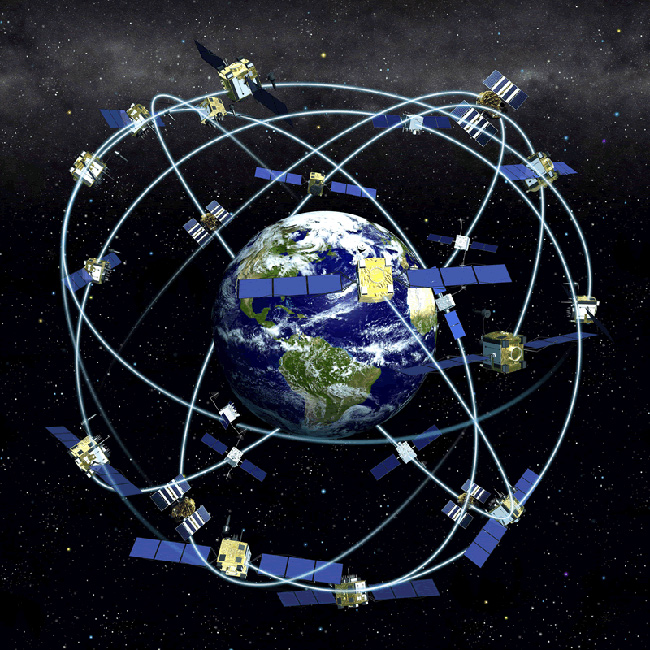
\includegraphics[width=0.15\textwidth]{Figures/gps_constellation_dark.jpg}
			};
			\node (cap2) [below=0cm of gps,xshift=2.7em,yshift=1.5em] {\textbf{Fig. 2}};
		\end{center}
		\vspace{1em}
		%
		\node (vlbi) [below=0cm of cap2,xshift=2.7em,yshift=2.0em] {
				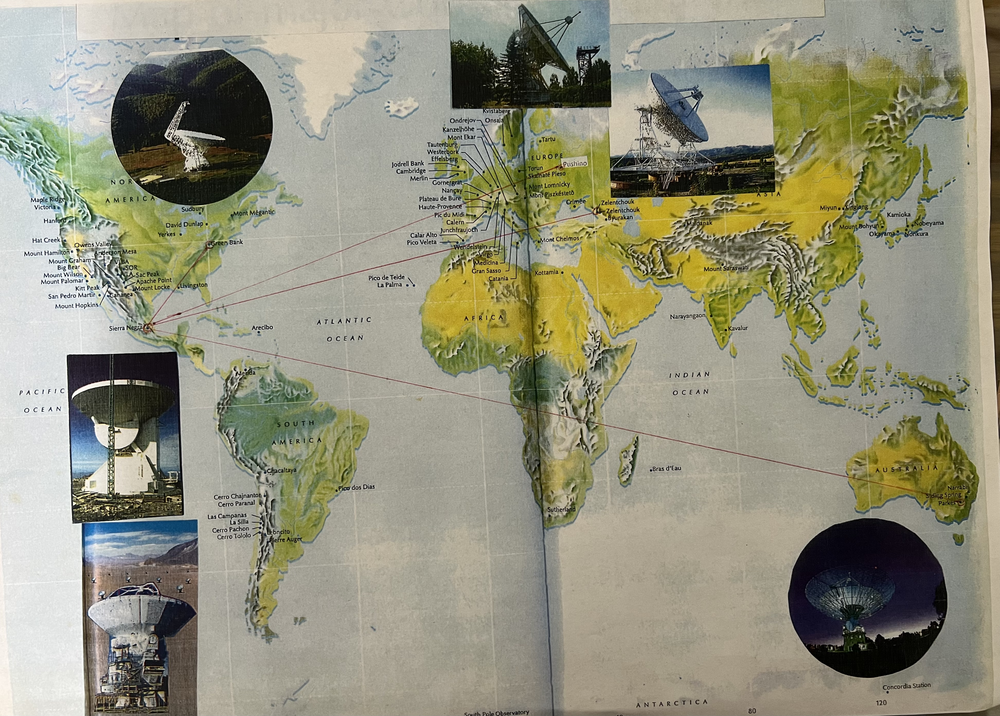
\includegraphics[width=0.20\textwidth]{Figures/VLBI_stations_proposal.png}
		};
		\node (cap4) [below=0cm of vlbi,xshift=2.7em,yshift=1.5em] {\textbf{Fig. 4}};
		\vspace{34em}
		%
	}
\end{subcolumns}

\block{}{
VLBI is viable in Mexico since the establishment of the GMT (owned by INAOE and UMass) provided a companion radiotelescope can be found.
Here we propose five possible companions:
Green Bank, Krym, Pushino, Parkes, and Alma,
whose positions are shown in Fig.~4.
For a preliminary evaluation of these baseline components we use the coordinates given in Tab.~1.
\vspace{1em}

The principle behind the use of interferometric observations of far away radiosources (quasars) is based on the fact that the quasar's signals (see Fig.~5) do not arrive at the same time to the antennas of the radiotelescopes $Q_1$ and $Q_2$ located at a great distance from each other (baseline).
The time difference is due to the difference in distance from each radiotelescope to the radiosource.
}

% Table and Fig.
\begin{subcolumns}
    \subcolumn{0.32} 
		\block{}{
			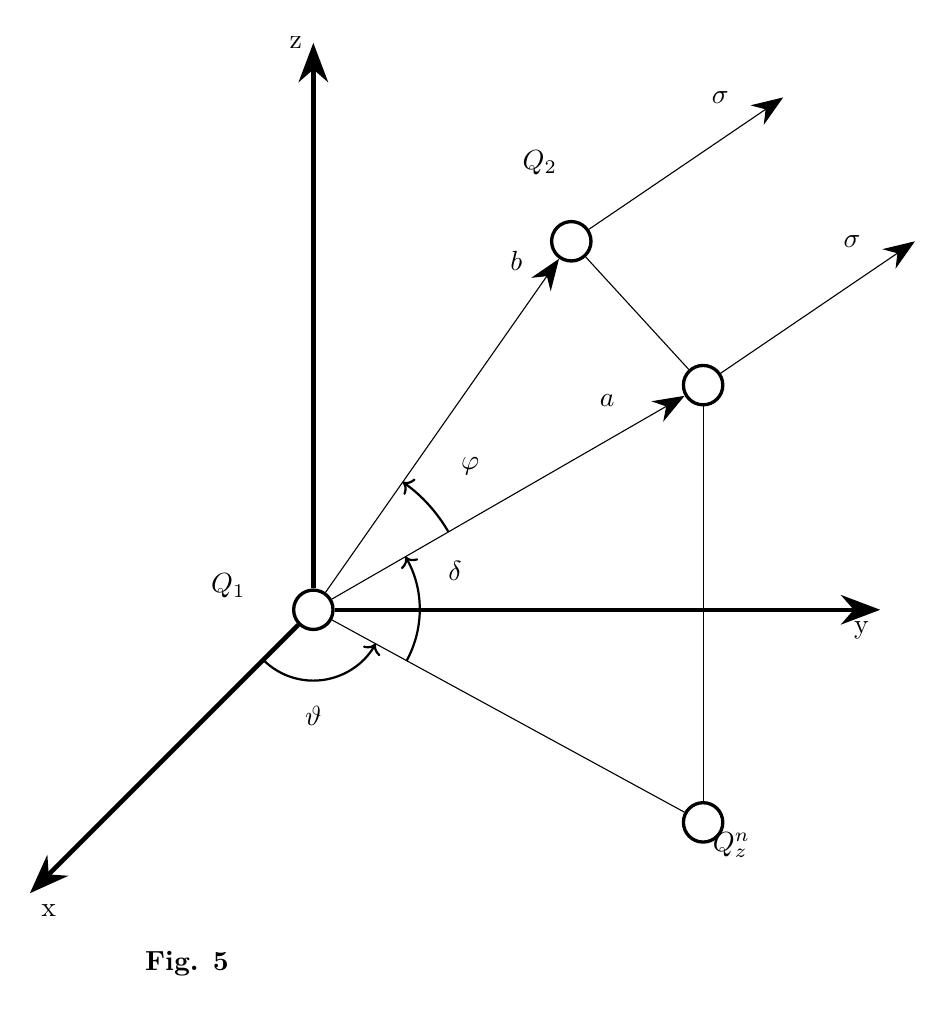
\begin{tikzpicture}[scale=0.9,
				roundnode/.style={circle, draw, very thick, inner sep=0pt, minimum width=5mm},
				]
				% Nodes
				\node[roundnode] (v0) at (0,0) {};
				\node[roundnode] (v1) at (5.5,-3.0) {};
				\node[roundnode] (va) at (5.5,3.17) {};
				\node[roundnode] (vb) at (3.64,5.20) {};

				% Axes
				\draw[ultra thick, -{Stealth[length=5mm]}] (v0) -- (0,8)
					node[anchor=east]{z};
				\draw[ultra thick, -{Stealth[length=5mm]}] (v0) -- (8,0) 
					node[anchor=north east]{y};
				\draw[ultra thick, -{Stealth[length=5mm]}] (v0) -- (-4,-4) 
					node[anchor=north west] (x-axis) {x};

				% Vectors
				\draw[-{Stealth[length=4mm]}] (v0) -- (va)
					node[anchor=north east,xshift=-1cm]{$a$};
				\draw[-{Stealth[length=4mm]}] (v0) -- (vb)
					node[anchor=north east,xshift=-5mm]{$b$};
				\draw[-{Stealth[length=4mm]}] (va) -- (8.49, 5.20);
				\draw[-{Stealth[length=4mm]}] (vb) -- (6.63, 7.23);

				% Connecting dots
				\draw (va) -- (vb) ;
				\draw (va) -- (v1) ;
				\draw (v0) -- (v1) node[anchor=north west]{$Q^n_z$};

				% Arcs
				\draw[thick, ->] (-0.707,-0.707) arc (225:331.389:1);
				\draw[thick, ->] (1.317,-0.718) arc (-28.610:29.958:1.5);
				\draw[thick, ->] (1.906,1.099) arc (29.958:55.008:2.2);

				% Labels
				\node[yshift=3mm] at (-1.2,0) {$Q_1$};
				\node[xshift=-4mm,yshift=10mm] at (3.64,5.20) {$Q_2$};
				\node[yshift=0mm] at (0,-1.5) {$\vartheta$};
				\node[yshift=5mm] at (2,0) {$\delta$};
				\node[yshift=0mm] at (2.212,2.026) {$\varphi$};
				\node[xshift=-8mm] at (8.49, 5.20) {$\sigma$};
				\node[xshift=-8mm] at (6.63, 7.23) {$\sigma$};

				% Fig label
				\normalsize
				\node (vlbi-scheme) [below=0cm of x-axis, xshift=5em, yshift=-0.5em] {\textbf{Fig. 5}}; 
			\end{tikzpicture}
		} 
    \subcolumn{0.68} 
			\block{}{
				\normalsize
				\begin{flushright}
					{\renewcommand{\arraystretch}{1.0}
						\renewcommand{\tabcolsep}{0.2cm}
						\begin{tabular}{| >{\centering\arraybackslash}p{4.5cm}|c|c|c|c|c|}
							\hline
							Station & 
							$\Lambda,$ deg & $\Phi,$ deg & $X,$ m & $Y,$ m & $Z,$ m \\ \hline
							Sierra Negra & 
							96W & 19 & $-6303374.17$ & $-5997609.56$ & 2076517.97 \\ 
							(0) & & & & & \\ \hline
							Green Bank & 
							78W & 39 & 1030564.74 & $-4848425.92$ & 4013891.04 \\ 
							(1) & & & & & \\ \hline
							Krim & 
							43E & 43 & 3411526.14 & 3181299.59 & 4349878.29 \\ 
							(2) & & & & & \\ \hline
							Puschino & 
							37E & 55 & 2921687.03 & 2201649.10 & 5224663.14 \\ 
							(3) & & & & & \\ \hline
							Parkes & 
							149E & $-34$ & $-4532455.87$ & 2723374.24 & $-356608.39$ \\
							(4) & & & & & \\ \hline
							ALMA & 
							\ang{70;24}W & \ang{24;24}S & 1948920.01 & $-5473203.27$ & $-2629980.09$ \\ 
							(5) & & & & & \\ \hline
						\end{tabular}
					}
					{
						\rule{0pt}{3ex}
						\textbf{Tab.~1\space\space 
							Coordinates of the radiotelescopes considered in this project}
					}
				\end{flushright}
			}
\end{subcolumns}

\block{}{
After submitting the abstract to COSPAR we found in: http://www.imfgtm.org,
that the VLBI capability of the GTM had been demonstrated by astronomers from 
INAOE, UMass, Haystack Observatory, MIT and NRAO, 
observing the quasar 1633+382 through VLBI at 3mm, 
using the GTM Alfonso Serrano on the summit of Sierra Negra, Puebla 
in combination with seven radiotelescopes located as shown on Fig.~6.
The fringes detected are shown Fig.~7.
}

\block{}{
	\normalsize
	\begin{center}
		\node[anchor=north west,xshift=-0.5em,yshift=1em] (locations) {
			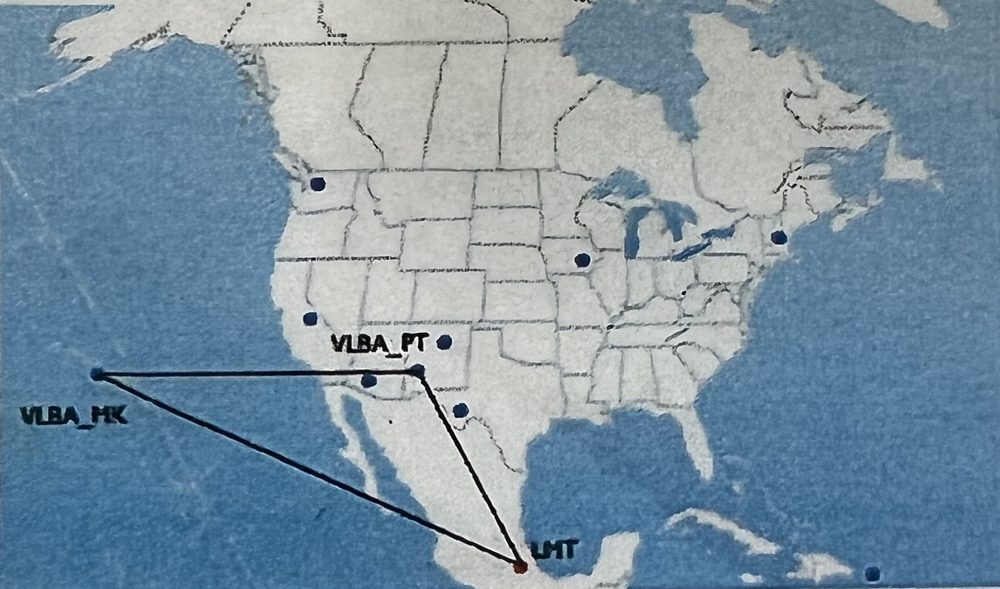
\includegraphics[height=0.15\textwidth]{Figures/locations_VLBI.png}
		};
		\node (cap6) [below=0cm of locations,xshift=2.7em,yshift=1.5em] {\textbf{Fig. 6}};
	\end{center}
	\vspace{1em}
	%
	\node (fringes) [right=of locations.north east, xshift=7.5em, yshift=-4em] {
		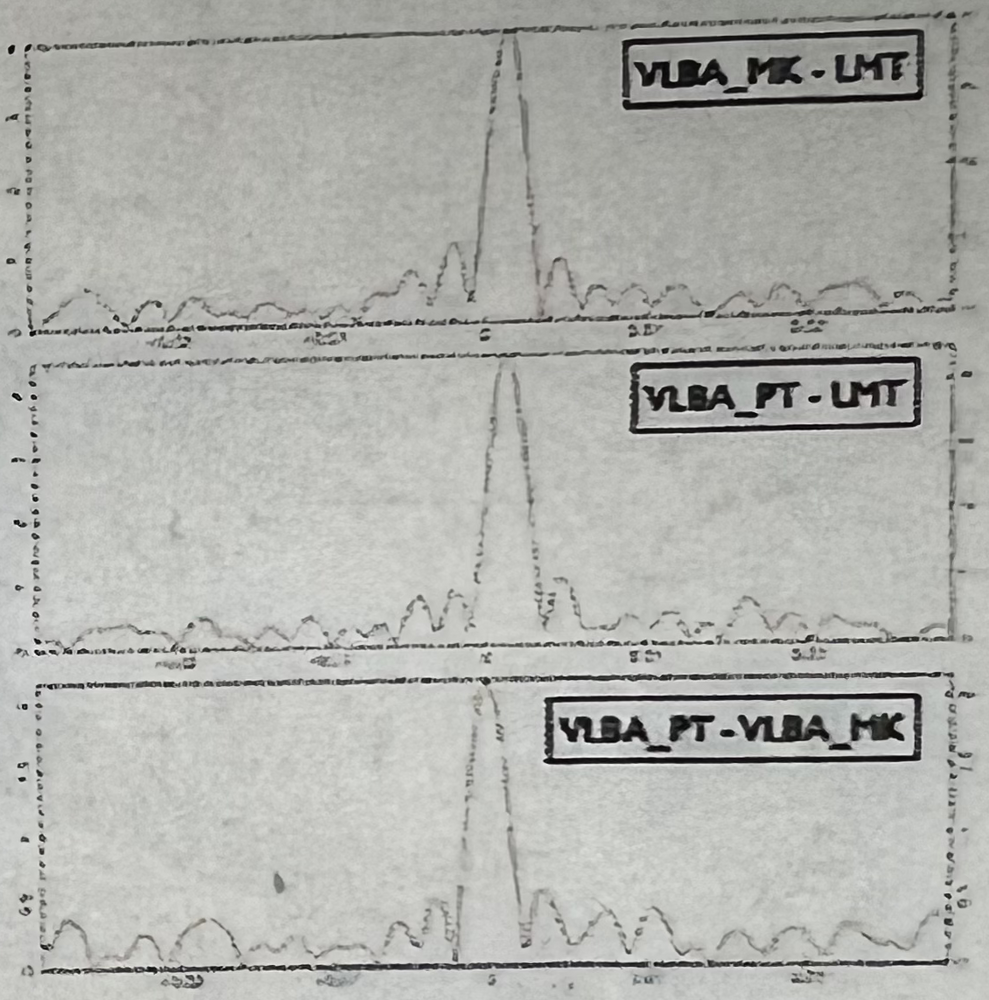
\includegraphics[height=0.15\textwidth]{Figures/fringes_vlbi.png}
	};
	\node (x-axis-7) [below=0cm of fringes,xshift=2.7em,yshift=1.5em] {
		\textbf{Fringe Delay Rate (ns/s)}
};
	\node (y-axis-7) [left=0cm of fringes, xshift=4.5em, yshift=11.0em, rotate=90] {
		\textbf{Correlation Amplitude (\mbox{\boldmath$\times 10^{-4}$})}
};
	\node (cap7) [below=0cm of x-axis-7, xshift=4.0em, yshift=2.5em] {\textbf{Fig. 7}};
	\vspace{11em}
	%
}

\block{}{

\textbf{References}
\vspace{1em}

1.-~Krilov~V.~I. 
Cosmic Geodesy. 
Ed. UPP Reprographia MIIGAIK,
p.168, 
Moscow 2002.

2.-~Prilepin~M.~T., Shanurov~G.~A. 
Radiointerferometry of Long Baselines and its Applications. 
Ed. Achievements of Science and Technology Series: Geodesy and Photogrametry, 
p. 66-105,
Moscow \mbox{BNIIFTRI} 1983.
}

 % Second column
\column{0.5}% Width set relative to text width

\block{}{
As an example,
let us consider the case for the Sierra Negra-Green Bank baseline.
The visibility zones for these radiotelescopes can be calculated with the following equation:
\begin{multline*}
	h_{ki} = \arcsin( \sin\Phi \sin(-90\degree + k\degree) + 
								\cos(-90\degree + k\degree) \cos\Phi \cos(i\degree - 
									\Lambda)
						), \\
	k = 0, 1, ..., 180; i = 0, 1, ..., 360.
\end{multline*}
}

\begin{subcolumns}
	% Left column image
	\subcolumn{0.5} 
	\block{}{
		\begin{tikzfigure}
			\node[anchor=north west, xshift=-0.5em, yshift=1.5em] (vis1) {
				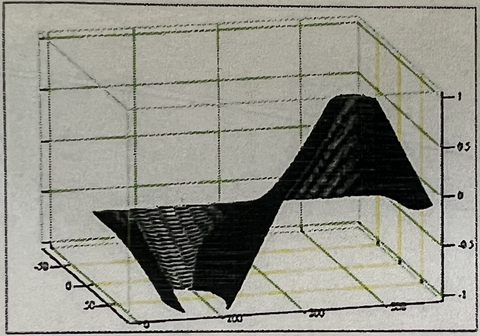
\includegraphics[height=0.14\textwidth]{
					Figures/visibility_zone_1.png
				}
			};
			\node (cap8) [below=0cm of vis1, xshift=2.5em, yshift=1.5em] {
				\textbf{Fig.~8. Visibility zone for the LMT}
			};
		\end{tikzfigure}
	} 
	% Right column image
	\subcolumn{0.5} 
	\block{}{
		\begin{tikzfigure}
			\node[anchor=north west, xshift=-3em, yshift=1.5em] (vis2) {
				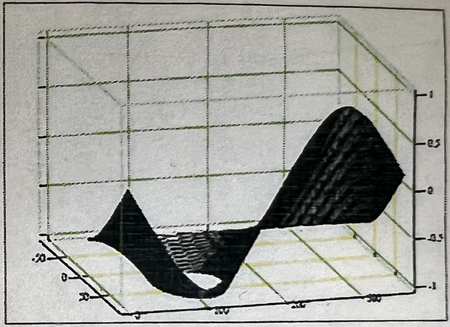
\includegraphics[height=0.14\textwidth]{
					Figures/visibility_zone_2.png
				}
			};
			\node (cap9) [below=0cm of vis2, xshift=2.4em, yshift=1.5em] {
				\textbf{Fig.~9. Visibility zone for Green Bank}
			};
		\end{tikzfigure}
		\vspace{11em}
	}
\end{subcolumns}

\block{}{
\begin{center}
	\textbf{Theory of the VLBI method}
	\vspace{1em}
\end{center}

Linking equation of the VLBI method:
\begin{equation*}
	c \tau = \Delta X_{ij} L + \Delta Y_{ij} M + \Delta Z_{ij} N,
\end{equation*}

where $L = \cos\gamma \cos\delta$,
$M = \sin\gamma \cos\delta$,
and $N = \sin\delta$.

Here, $\gamma$ and $\delta$ are the spherical coordinates of the quasars, where
\begin{equation}
	A = 
		\begin{pmatrix}
			L_1 & M_1 & N_1 \\
			\vdots & \vdots & \vdots \\
			L_n & M_n & N_n \\
		\end{pmatrix},
\end{equation}

\begin{equation*}
	\vec X = 
		\begin{pmatrix}
		 	\delta \Delta X \\
			\delta \Delta Y \\
			\delta \Delta Z \\
		\end{pmatrix},
\end{equation*}

\begin{equation*}
	\vec L = 
		\begin{pmatrix}
			c \tau^{(c)}_1 - \tau^{(0)}_1 \\
			\vdots \\
			c \tau^{(c)}_n - \tau^{(0)}_n \\
		\end{pmatrix},
\end{equation*}

\begin{equation*}
	\vec \nu = 
		\begin{pmatrix}
			\nu_1 \\
			\vdots \\
			\nu_n \\
		\end{pmatrix}.
\end{equation*}

Normal equations
\begin{equation*}
	A^T A \vec X  + A^T \vec L = 0.
\end{equation*}

Solution
\begin{equation*}
	\vec X = -(A^T A)^{-1} A^T L.
\end{equation*}

The precision evaluation is:
\begin{IEEEeqnarray*}{rCl}
	\mu & = & \sqrt{\frac{{\vec \nu}^T \nu}{n - 3}}, \\
	Q = (A^T A)^{-1} & = & 
		\begin{pmatrix} 
			q_{xx} & q_{xy} & q_{xz} \\
			q_{yx} & q_{yy} & q_{yz} \\
			q_{zx} & q_{zy} & q_{zz}
		\end{pmatrix}, \\ 
	m_{\Delta X} = \mu \sqrt{q_{xx}},
	m_{\Delta Y} & = & \mu \sqrt{q_{yy}},
	m_{\Delta Z} = \mu \sqrt{q_{zz}}.
	\vspace{0.5em}
\end{IEEEeqnarray*}

\textbf{\noindent
	A priori evaluation of the increments {\boldmath$\Delta X$}, {\boldmath$\Delta Y$}, and {\boldmath$\Delta Z$} on the basis of the VLBI.
	Base Sierra Negra - Green Bank. 
	Distance: 2798706.05m.
}

% Table
% Give the table more room
\vspace{1em}
\begin{center}
	\normalsize
	{\renewcommand{\arraystretch}{1.0}
		\renewcommand{\tabcolsep}{0.4cm}
		\begin{tabular}{|p{2cm}|l|l|l|l|l|l|l|l|l|l|}
			\multicolumn{11}{c}
			{Tab.~2\space\space Spherical coordinates of the quasars} \\
			\hline
			$\gamma$, deg & 
			0 & 185 & 190 & 195 & 200 & 205 & 210 & 215 & 230 & 240 \\ \hline
			$\delta$, deg & 
			85 & 86 & 78 & 70 & 62 & 56 & 50 & 46 & 36 & 31 \\ \hline
			$h0$, deg & 
			18 & 20 & 22 & 25 & 29 & 33 & 37 & 42 & 56 & 65 \\ \hline
			$h1$, deg & 
			40 & 38 & 38 & 36 & 37 & 38 & 40 & 42 & 49 & 55 \\ \hline
			$\gamma$, deg & 
			255 & 260 & 280 & 295 & 305 & 320 & 335 & 345 & 355 & 350 \\ \hline
			$\delta$, deg & 
			26 & 23 & 42 & 35 & 37 & 42 & 51 & 62 & 76 & 55 \\ \hline
			$h0$, deg & 
			79 & 85 & 63 & 58 & 50 & 38 & 27 & 21 & 18 & 18 \\ \hline
			$h1$, deg & 
			64 & 65 & 87 & 79 & 72 & 61 & 52 & 46 & 42 & 43 \\ \hline
	\end{tabular}}
\end{center}
\vspace{1em}

Measurement error \qquad $\sigma_\tau = 0.1$~nanosec. \\
Solution
\begin{IEEEeqnarray*}{C}
	\delta \Delta X = \qty{99.976}{m}; \quad
	\delta \Delta Y = \qty{-70.014}{m}; \quad
	\delta \Delta Z = \qty{50.007}{m}. \\
	m_{\Delta X} = \qty{.023}{m}; \quad
	m_{\Delta Y} = \qty{.024}{m}; \quad
	m_{\Delta Z} = \qty{.015}{m}.
\end{IEEEeqnarray*} 

Model values: 
{\boldmath$
	\Delta X = \qty{1660938.908}{m}, \, 
	\Delta Y = \qty{1149183.641}{m}, \, 
	\Delta Z = \qty{1937373.075}{m}. \,
$}

Approximate values:
{\boldmath$
	\Delta Y = \qty{1149253.641}{m}, \, 
	\Delta Z = \qty{1937323.075}{m}. \,
$}


}

\block{}{
\textbf{Conclusion:}
VLBI is viable with the GTM as proposed here, and in fact it has already been demonstrated by INAOE and several US astronomical institutions which are planning to use it for relevant astronomical applications. 
We would like to emphasize, however, the importance of using it for the ITRF as presented here.
This project would additionally allow the participation of medium size universities in Mexico like UAS and UNISON,
as well as to foster international collaborations,
such as the ones considered here:
Zelenchuk, Pushino (Russia), 
Green Bank (USA),
Parkes (Australia), 
and
Alma (Chile).
}

\end{columns}

\end{document}
